\documentclass[]{book}
\usepackage{lmodern}
\usepackage{amssymb,amsmath}
\usepackage{ifxetex,ifluatex}
\usepackage{fixltx2e} % provides \textsubscript
\ifnum 0\ifxetex 1\fi\ifluatex 1\fi=0 % if pdftex
  \usepackage[T1]{fontenc}
  \usepackage[utf8]{inputenc}
\else % if luatex or xelatex
  \ifxetex
    \usepackage{mathspec}
  \else
    \usepackage{fontspec}
  \fi
  \defaultfontfeatures{Ligatures=TeX,Scale=MatchLowercase}
\fi
% use upquote if available, for straight quotes in verbatim environments
\IfFileExists{upquote.sty}{\usepackage{upquote}}{}
% use microtype if available
\IfFileExists{microtype.sty}{%
\usepackage{microtype}
\UseMicrotypeSet[protrusion]{basicmath} % disable protrusion for tt fonts
}{}
\usepackage{hyperref}
\hypersetup{unicode=true,
            pdftitle={Experimentum: Web-based Software for Psychology Studies},
            pdfauthor={Rebecca J. Lai, Rifah Abdullah, Gaby Mahrholz, Lisa DeBruine},
            pdfborder={0 0 0},
            breaklinks=true}
\urlstyle{same}  % don't use monospace font for urls
\usepackage{natbib}
\bibliographystyle{apalike}
\usepackage{longtable,booktabs}
\usepackage{graphicx,grffile}
\makeatletter
\def\maxwidth{\ifdim\Gin@nat@width>\linewidth\linewidth\else\Gin@nat@width\fi}
\def\maxheight{\ifdim\Gin@nat@height>\textheight\textheight\else\Gin@nat@height\fi}
\makeatother
% Scale images if necessary, so that they will not overflow the page
% margins by default, and it is still possible to overwrite the defaults
% using explicit options in \includegraphics[width, height, ...]{}
\setkeys{Gin}{width=\maxwidth,height=\maxheight,keepaspectratio}
\IfFileExists{parskip.sty}{%
\usepackage{parskip}
}{% else
\setlength{\parindent}{0pt}
\setlength{\parskip}{6pt plus 2pt minus 1pt}
}
\setlength{\emergencystretch}{3em}  % prevent overfull lines
\providecommand{\tightlist}{%
  \setlength{\itemsep}{0pt}\setlength{\parskip}{0pt}}
\setcounter{secnumdepth}{5}
% Redefines (sub)paragraphs to behave more like sections
\ifx\paragraph\undefined\else
\let\oldparagraph\paragraph
\renewcommand{\paragraph}[1]{\oldparagraph{#1}\mbox{}}
\fi
\ifx\subparagraph\undefined\else
\let\oldsubparagraph\subparagraph
\renewcommand{\subparagraph}[1]{\oldsubparagraph{#1}\mbox{}}
\fi

%%% Use protect on footnotes to avoid problems with footnotes in titles
\let\rmarkdownfootnote\footnote%
\def\footnote{\protect\rmarkdownfootnote}

%%% Change title format to be more compact
\usepackage{titling}

% Create subtitle command for use in maketitle
\providecommand{\subtitle}[1]{
  \posttitle{
    \begin{center}\large#1\end{center}
    }
}

\setlength{\droptitle}{-2em}

  \title{Experimentum: Web-based Software for Psychology Studies}
    \pretitle{\vspace{\droptitle}\centering\huge}
  \posttitle{\par}
    \author{Rebecca J. Lai, Rifah Abdullah, Gaby Mahrholz, Lisa DeBruine}
    \preauthor{\centering\large\emph}
  \postauthor{\par}
      \predate{\centering\large\emph}
  \postdate{\par}
    \date{2020-01-23}

\usepackage{booktabs}

\begin{document}
\maketitle

{
\setcounter{tocdepth}{1}
\tableofcontents
}
\hypertarget{about-experimentum}{%
\chapter*{About Experimentum}\label{about-experimentum}}
\addcontentsline{toc}{chapter}{About Experimentum}

\hypertarget{support}{%
\subsection*{Getting Support}\label{support}}
\addcontentsline{toc}{subsection}{Getting Support}

\hypertarget{for-experimentum-university-of-glasgow-users}{%
\subsubsection*{For Experimentum @ University of Glasgow Users}\label{for-experimentum-university-of-glasgow-users}}
\addcontentsline{toc}{subsubsection}{For Experimentum @ University of Glasgow Users}

Currently there are two active admins available to provide support, these are \href{mailto:rebecca.lai@glasgow.ac.uk}{Rebecca Lai} and \href{mailto:lisa.debruine@glasgow.ac.uk}{Professor Lisa DeBruine}.

Admins play a double role. In addition to helping you with Experimentum we are active researchers and teaching staff with additional jobs to do elsewhere. Our inboxes are often full, and emails will often go unread.

As a result of this, all students and staff who are experiencing technical issues should use the Slack workspace \href{https://experimentum-web.slack.com/}{``Experimentum-web''} to get support. Additionally, we are using the queries on the slack workspace to best update the user documentation, so it is important to keep all correspondence in one neat location.

\begin{rainbow}
You should never post data on this workspace, either in data file or
screenshot form, as this would be a violation of the GDPR. All such
files will be removed and your supervisor will be informed.

If you need to share your data please use one of the university approved
services available to you, such as OneDrive or OwnCloud.
\end{rainbow}

\hypertarget{lost-passwords}{%
\subsection*{Lost Passwords}\label{lost-passwords}}
\addcontentsline{toc}{subsection}{Lost Passwords}

For security reasons we do not allow users to request a password reset automatically.

If you are any type of account holder who has lost their password, please contact the admins or your supervisor to ask for it to be reset. This request should only be honoured if sent from the email address associated with the account. A temporary password will be issued, which is case-sensitive, and should be changed as soon as possible.

For accounts types which have access to participant data (student \& researcher), contact your supervisor or admins. Be prepared to visit with your student card to have your password reset.

\hypertarget{changing-your-password}{%
\subsection*{Changing Your Password}\label{changing-your-password}}
\addcontentsline{toc}{subsection}{Changing Your Password}

You can change your password by signing in, navigating to ``My Account'' from the menu on the right of the page and clicking the link ``change your password'' under ``Username'':

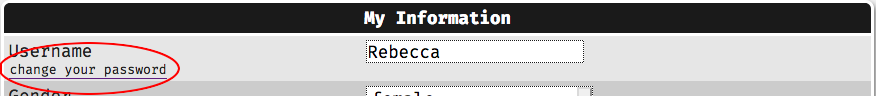
\includegraphics{images/screenshots/change_password.png}

\hypertarget{tutorial-sessions}{%
\paragraph{Tutorial Sessions}\label{tutorial-sessions}}
\addcontentsline{toc}{paragraph}{Tutorial Sessions}

During times of particularly heavy use through the academic year we may schedule specific help sessions to deal with common issues and to help you fix specific problems that you might have. These will be advertised on the Slack workspace and on appropriate Moodle pages.

If you are experiencing an issue that is particularly difficult to fix remotely, you can make an appointment with Rebecca via private message on the \href{https://experimentum-web.slack.com/}{``Experimentum-web''} workspace. However, you should have made attempts to solve the issue remotely first as time available for these appointments is extremely limited.

If you require assistance to navigate this document or create your study due to disability please contact your supervisor who may refer you to the admins.

\hypertarget{for-other-users}{%
\subsubsection*{For Other Users}\label{for-other-users}}
\addcontentsline{toc}{subsubsection}{For Other Users}

If you download and use the code for this platform you should establish clear guidelines outlining the role of the admins and methods of support in accordance with any relevant regulations.

Staff from the University of Glasgow will not provide support for users of other systems based upon this code. Our Slack workspace is for internal use only.

If you find an issue with the Experimentum codebase, please file an issue \href{https://github.com/debruine/experimentum/issues}{here}. If you find an issue with the codebase for this manual you can file an issue \href{https://github.com/RebeccaJLai/exp_manual/issues}{here}.

\hypertarget{privacy-notices}{%
\section*{Privacy Notices}\label{privacy-notices}}
\addcontentsline{toc}{section}{Privacy Notices}

\hypertarget{cookies}{%
\subsection*{Cookies}\label{cookies}}
\addcontentsline{toc}{subsection}{Cookies}

Cookies are used for Experimentum to allow us to track user sessions, which allows participants to navigate between pages during a session without having to log in to every page. In the case of anonymous logins, the session is tracked to maintain the same identity across multiple elements of the same study.

Cookies are not tracked beyond a single session, for either registered or anonymous participants. By closing the browser the current session is ended and cookies tracking the session are discarded.

Cookies are not used in any other way by us, and the information is not retained or shared with any other organisations.

\hypertarget{data-management}{%
\subsection*{Data Management}\label{data-management}}
\addcontentsline{toc}{subsection}{Data Management}

Your study's data is your responsibility. Please ensure that it is protected and used appropriately. University of Glasgow guidelines with regard to data protection are available to view \href{https://www.gla.ac.uk/myglasgow/dpfoioffice/}{here} and more general data management guidelines \href{https://www.gla.ac.uk/myglasgow/datamanagement/rdmatglasgow/}{here}.

Experimentum saves your data to the University of Glasgow School of Psychology secure servers, which are on-site in Hillhead Street. Data will be output in Comma Separated Value (.csv) files in ``tidy'' format and is available for download from by the researcher(s) who own the study, their supervisors and admins \textbf{only}.

Whilst data processing questions should be directed to the researcher (or your supervisor(s) and advisors if you are a student/researcher), there are a couple of common tasks that you might find yourself needing to do. See the examples in the section \protect\hyperlink{commoncode}{Commonly used R code} for help with some common code segments.

\hypertarget{about-your-data}{%
\subsection*{About your data}\label{about-your-data}}
\addcontentsline{toc}{subsection}{About your data}

With all account types, besides anonymous participation, your user ID is linked to the data that you submit. This allows us to track users in multi-part studies, but it also means that our servers will contain multiple bits of information about you built up through your participation.

Individual researchers will only be able to access the data that you submit on their studies, and not data you submit to studies belonging to other researchers. In real terms, this means that individual researchers will only see the data that you give to them, not the data that you give across the entire site.

In cases where you participate in multiple studies for the same researcher, they will be able to see your data across these studies. Individual researchers are responsible for the protection of your privacy, ensuring that there is no way for any third party to use this information to ``triangulate'' your identity using the information you have provided.

If you have any concerns about how your data is used please contact the researchers involved in the study or studies that you are taking/have taken part in. To see the University's guidelines on how researchers should treat data see \href{https://www.gla.ac.uk/myglasgow/dpfoioffice/}{here}.

\begin{warning}
You have rights concerning your own data and how it is used, and
responsible researchers should always hold these in the highest regard.

If you have any concerns about how your data is being used you should
contact the researcher in question in the first instance.

If you are reluctant to speak to them directly you can speak to their
supervisor, whose contact information should be given to you at the time
of undertaking the study or upon request from the researcher.

Alternatively, you can contact the Data Protection and Freedom of
Information Office
\href{https://www.gla.ac.uk/myglasgow/dpfoioffice/contact/}{here}.
\end{warning}

\hypertarget{consent}{%
\subsection*{Consent}\label{consent}}
\addcontentsline{toc}{subsection}{Consent}

Upon registration, users are asked to complete a standardised consent form:

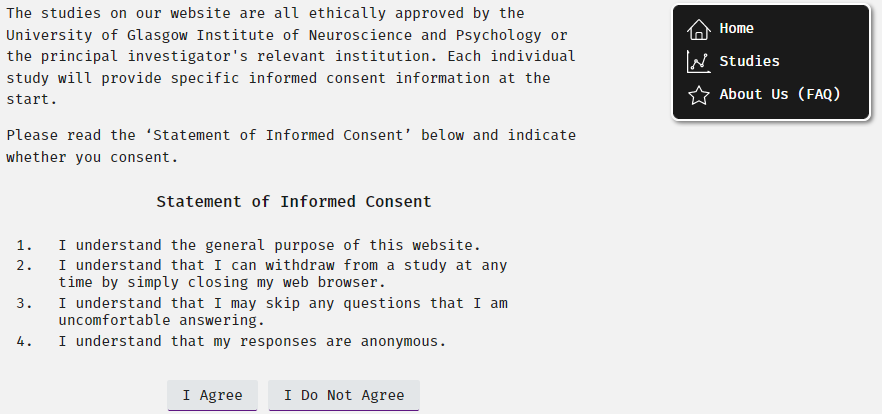
\includegraphics{images/screenshots/consent.png}

When constructing studies, you should also include your own consent form, including all relevant information specified by your supervisor(s) and regulatory body relevant to your work.

\hypertarget{codebase}{%
\section*{Codebase}\label{codebase}}
\addcontentsline{toc}{section}{Codebase}

Open code for the site and installation instructions are available to download \href{https://github.com/debruine/experimentum}{here}. This is provided under a \href{https://creativecommons.org/licenses/by-sa/3.0/legalcode}{CC-BY-SA 3.0} license.

The same is provided for this user guide \href{https://github.com/RebeccaJLai/exp_manual}{here}, and under this same \href{https://creativecommons.org/licenses/by-sa/3.0/legalcode}{license}. This document was authored using bookdown \citep{R-bookdown}. See \href{https://bookdown.org/yihui/bookdown/}{here} for instructions on making modifications, rendering and publishing such documents.

\hypertarget{acknowledgements}{%
\section*{Acknowledgements}\label{acknowledgements}}
\addcontentsline{toc}{section}{Acknowledgements}

\begin{tabular}{l|l}
\hline
Our thanks to: &  \\
\hline
Gaby Mahrholtz: & For bug hunting and fruitful discussion on workarounds and best practice.\\
\hline
Dr Niamh Stack: & For support in the development of the user guide.\\
\hline
\end{tabular}

\hypertarget{quick-start-guide}{%
\chapter{Quick Start Guide}\label{quick-start-guide}}

\hypertarget{the-bare-essentials}{%
\section{The Bare Essentials}\label{the-bare-essentials}}

\hypertarget{accounts}{%
\chapter{User Accounts}\label{accounts}}

\hypertarget{overview}{%
\section{Overview}\label{overview}}

There are several account types that you can have with Experimentum, each with its own purpose and different levels of privileges.

This chapter explains what account types exist, what they do, which type of account you might want to have and how to change account types for supervisors.

\hypertarget{account-types}{%
\section{Account Types}\label{account-types}}

\hypertarget{guest-accounts}{%
\subsection{``Guest'' Accounts}\label{guest-accounts}}

For participants who are not required to have an account. You do not need to be signed in but you can still take part in some experiments on the site. When you close your browser, this account is discarded and no longer tracked. This allows for anonymous participation in some experiments.

\begin{warning}
If a guest participant closes their browser mid-way through a study
their progress will not be saved and the data will read as an incomplete
run.
\end{warning}

As guest users do not have a profile, we do not store their age, gender or any other types of information about them. We suggest that you do not place age or gender restrictions on studies where participants take part anonymously as guests. When guests sign into a study with age or gender restrictions, they will see a dialogue box asking them for their age and gender.

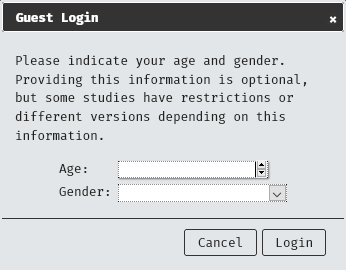
\includegraphics{images/screenshots/guest_dialogue.png}

This information is used to prevent those who should not take part from taking part and inserted into the user information in the downloaded data files. If you need to collect further demographic information, we suggest constructing a demographics questionnaire component.

\hypertarget{registered-accounts}{%
\subsection{``Registered'' Accounts}\label{registered-accounts}}

These accounts are for participants. You have created an account and given us your date of birth and gender identification. You can participate in studies on the site. Your participation record is tracked, meaning that you can be linked across multiple-part studies.

Under no circumstances should you be linked across multiple studies without your explicit permission, we will never use data to ``triangulate'' your identity. Researchers can only access your data from their own studies, not the studies of other researchers.

\hypertarget{student-accounts}{%
\subsection{``Student'' Accounts}\label{student-accounts}}

For students who are conducting research as part of a mini project, undergraduate dissertation, master's or doctoral thesis. To create and run studies you must first register and then request researcher status.

Your supervisor will be the person who changes your account status and you can check the status of your account by looking at your account info. When approved, students will be given ``student'' status, a special type of research account.

You may still use this account to participate in experiments, but we advise setting up a separate registered, non-research account for participation to prevent serious data submissions from being removed by other investigators.

\hypertarget{researcher-accounts}{%
\subsection{``Researcher'' Accounts}\label{researcher-accounts}}

For staff, more senior students and anyone who may be supervising students using Experimentum. Follow the instructions for students as above, but staff should set either Lisa DeBruine or Rebecca Lai as their supervisor, who will grant them ``researcher'' status.

If you plan on supervising students using Experimentum you should set up a researcher account to be able to oversee the construction of their studies, share components and change studies to ``active'' before data collection can begin.

When you have established your researcher account your name will appear in the list of potential supervisors for students to choose from.

\begin{warning}
Supervisors should have a researcher account if they intend for their
students to use this system.

Supervision duties in this system should not be passed to another member
of staff so that you can avoid registering. Admins will not accept any
of the duties of the supervisor.

See the \protect\hyperlink{roles}{Supervisor Cheatsheet} for a breakdown
of the roles of the admins and the supervisors.
\end{warning}

\hypertarget{test-accounts}{%
\subsection{``Test'' Accounts}\label{test-accounts}}

For students and staff. This account type gives you the same amount of privileges as the registered account for participants, but any data collected from these accounts is saved in data sets with a status of ``test''.

This allows you and other test accounts to try out your study and easily identify and filter out which data should be excluded from the analysis. If you wish to have a test account contact an admin to set this up.

\hypertarget{admin-accounts}{%
\subsection{``Admin'' Accounts}\label{admin-accounts}}

For staff who assist others constructing and managing their studies online. This is the highest level of access.

An admin account basically allows us to ``supervise'' all users, including researcher accounts. We use this to see what is happening when problems arise to help provide aid, not to take responsibility for approval of status changes of students or oversee the design or activation of studies.

\hypertarget{registration-process}{%
\section{Registration Process}\label{registration-process}}

In order to sign up to the site you will select ``Sign up'' on the top right-hand side of the page. Once there you will be taken to a new page as below and asked to create a username, set a password and confirm it, provide your gender identity and birthday. Completing these steps alone will create a ``registered'' account type.

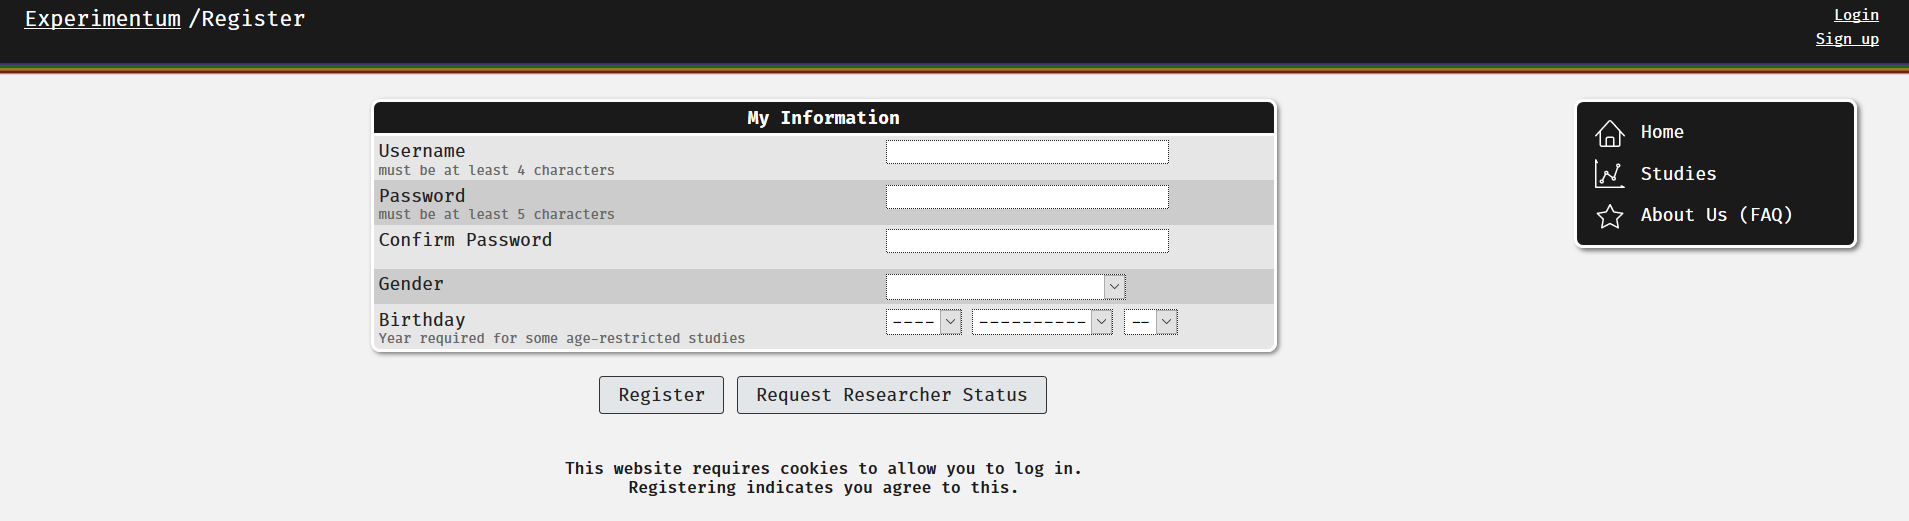
\includegraphics{images/screenshots/register.png}

With this account type you can participate in studies on the site. Your participation record is tracked, meaning that you can be linked across multiple-part studies. Under no circumstances will you be linked across multiple studies without your explicit permission and we will never use data to ``triangulate'' your identity. Researchers and students can only access your data from their own studies, not the studies of others.

\hypertarget{requesting-researcher-status}{%
\section{Requesting Researcher Status}\label{requesting-researcher-status}}

If you are a researcher or a student who is using the site to conduct a research project (such as a mini or maxi project, or an MSc or PhD thesis) you will need to request permission to construct and conduct studies. If you are a supervising member of teaching staff, you will also need to have an account in order to supervise your students project.

On the registration page, or the account page if you have already registered, there is a ``Request Researcher Status'' button. When you click on this additional fields will appear that you will need to fill in, as below.

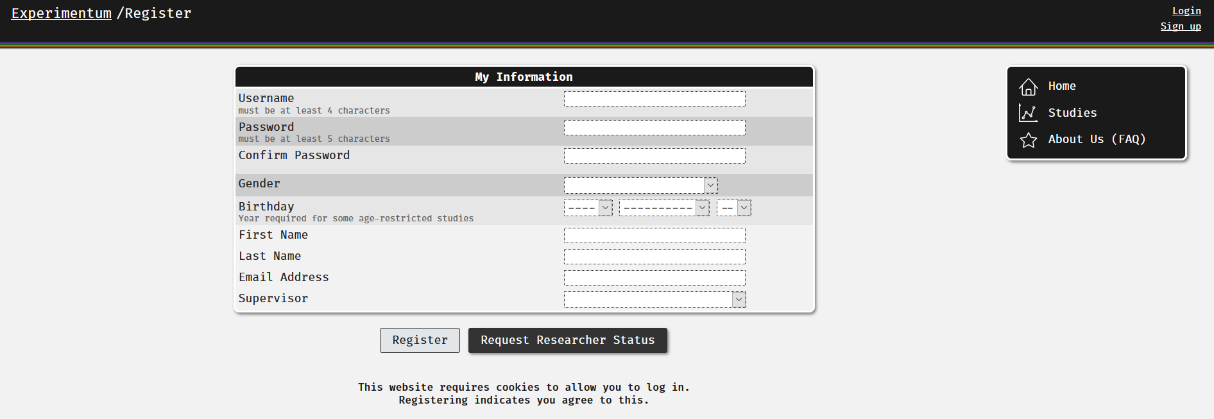
\includegraphics{images/screenshots/requesting_status.png}

You will need to provide us with your name, your email address and your supervisor. You should use your university email address to sign up and provide your real name so that your supervisor can more easily identify you. If you are a student conducting a research project you should select the member of staff supervising your project from the drop-down menu of supervisors.

\begin{info}
If you are a supervising member of teaching or research staff, you
should request Lisa DeBruine or Rebecca Lai as your supervisor.

If you are a more senior student who is relatively self-sufficient or
you have supervising duties of your own, \emph{and your supervisor
agrees to it}, you can also request Lisa or Rebecca as your supervisor,
and we will set you as a ``researcher'' account type.

As a general rule, all students completing a research project should be
assigned ``student'' status. Some PhD students may be better off with
``researcher'' status. Such individuals should speak to their
supervisors and the admins to determine which is the best account type
for them.
\end{info}

\hypertarget{checking-your-account-status}{%
\section{Checking your account status}\label{checking-your-account-status}}

When you first sign up your account will be the ``registered'' type and will remain as such until your researcher status is approved.

You can check on the status of your account by selecting ``account'' from the menu on the right-hand side of the page. Underneath the ``My Information'' section of the page will tell you your date of registration, number of logins and current account type.

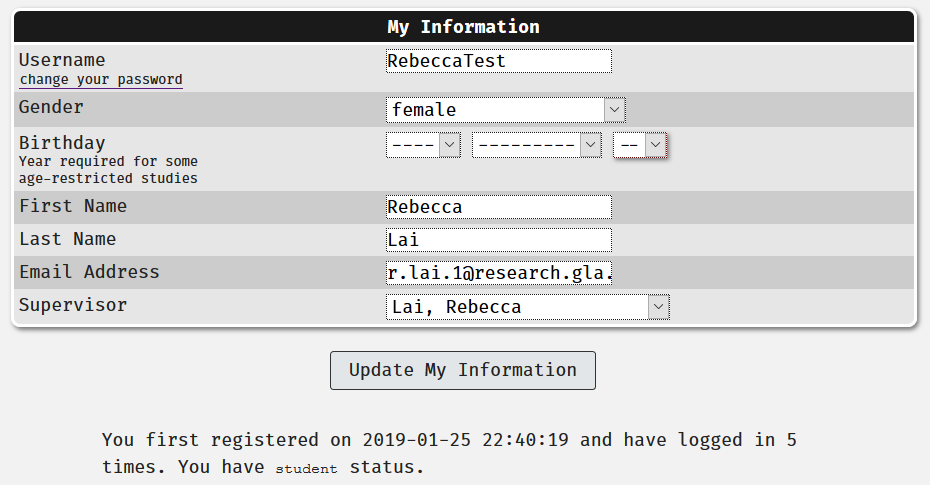
\includegraphics{images/screenshots/check_status.png}

The menu on the right also changes when you have been granted researcher status, with a new option of ``Researchers'' available which takes you to the study creation area of the site.

\begin{info}
If there is a delay in accepting your request you should contact your
supervisor directly and not the admin staff. It is the responsibility of
the supervisor to make changes to your access level.

If your supervisor is experiencing technical difficulties in accepting
your request, they should contact the admins directly \emph{themselves}.
Admins will not respond to a student who is requesting help on behalf of
their supervisor.
\end{info}

\hypertarget{approving-student-and-researcher-status-requests}{%
\section{Approving Student and Researcher Status Requests}\label{approving-student-and-researcher-status-requests}}

Supervisors have a responsibility to ensure that their students have the status that they require to carry out their projects. This includes assigning them sufficient permissions to construct and deploy their studies.

Once the supervisor has ``researcher'' status they will have a new area of the website opened to them, accessible through the researchers' link in the menu on the right, which will contain a section called ``Admin'':

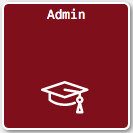
\includegraphics{images/screenshots/admin_button.png}

Clicking on this button will take them to a page with more options. To see and make changes to the privileges of those who have requested you as a supervisor and requested researcher status select the option ``Supervision'' from the menu.

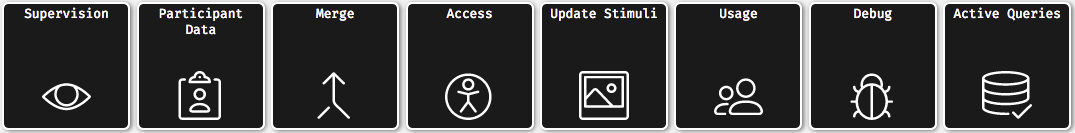
\includegraphics{images/screenshots/admin_options.png}

Here you will see a list of individuals who have requested you as a supervisor. To change their status, select the appropriate account type from the right-most drop-down menu under the column ``Status''.


\includegraphics{images/screenshots/status_bar.png}

The account you are making changes to will have to log out and back in again to be updated with their new permissions. When you press ``Send'' an email will be sent to the student to inform them of the status change.

\begin{bug}
There is a known issue with changing the statuses of research accounts
regarding accounts not being found by the system,
\protect\hyperlink{notfound}{see here}
\end{bug}

\hypertarget{stimuli}{%
\chapter{Stimuli}\label{stimuli}}

\hypertarget{overview-1}{%
\section{Overview}\label{overview-1}}

This chapter will cover how to upload your own stimuli, tips on naming conventions for the easiest possible way to assign stimuli to trials, accepted file formats and a rough guide to how to convert to the required formats.

\begin{warning}
Remember that not all image, video and audio files are free for use.
Check the license and terms of use of the images before you save, edit
or copy and paste them.
\end{warning}

\hypertarget{accepted-file-formats}{%
\section{Accepted File Formats}\label{accepted-file-formats}}

Experimentum uses what we hope to be the most universally applicable file formats to deliver your study.

These are the file formats that can be successfully displayed through the site. Please ensure that you conform to these types as others may not be tolerated by the system.

\begin{tabular}{l|l}
\hline
Stimuli Type & Accepted Formats\\
\hline
Images & JPEG, GIF and PNG\\
\hline
Audio & MP3\\
\hline
Video & M4V\\
\hline
\end{tabular}

\hypertarget{naming-conventions}{%
\section{Naming Conventions}\label{naming-conventions}}

In order to make the process of assigning stimuli to trials as easy as possible it is recommended that you establish a systematic way of assigning names to files.

The stage of assigning stimuli to trials goes much faster and smoother if you can search for the stimuli files names using some sort of common text string in the names of the files.

****** more info and a working example is required.

\hypertarget{pre-processing}{%
\section{Pre-Processing}\label{pre-processing}}

In order to get your stimuli up with the minimal amount of fuss, please ensure that you do any required pre-processing.

\hypertarget{images}{%
\subsection{Images}\label{images}}

Images should be of uniform size and of the correct file formats before uploading.

\hypertarget{converting-images}{%
\subsubsection*{Converting Images}\label{converting-images}}
\addcontentsline{toc}{subsubsection}{Converting Images}

GNU Image Manipulation Program \citep[``GIMP'',][]{gimp} is a free software that allows you to modify and export image files to a variety of file formats.


\includegraphics{images/screenshots/gimp.png}

This software was developed as a free and open source equivalent to photo-editing software such as Adobe Photoshop and can achieve very complex tasks. However, there are only 3 basic operations that you should be able to perform in GIMP order to convert your images to the correct formats. More complex operations are beyond the scope of this tutorial, but there are plenty of resources online should you choose to want to look them up.

If there are any further instructions that would prove helpful please file an issue \href{https://github.com/RebeccaJLai/exp_manual/issues}{here} describing what you want me to include in future versions of the manual.

\hypertarget{importing-images}{%
\paragraph{Importing Images}\label{importing-images}}
\addcontentsline{toc}{paragraph}{Importing Images}

There are a number of ways that you can import images into GIMP.

\hypertarget{file-open}{%
\subparagraph{File \textgreater{} Open}\label{file-open}}
\addcontentsline{toc}{subparagraph}{File \textgreater{} Open}

This is the simplest way to open an image file in GIMP.

Open the software first from your Start Menu or Launchpad. Then click on File \textgreater{} Open\ldots{}

***** image in here

A dialogue box will appear from which you can navigate to the location of the file you are attempting to open and select it. Click Open and the file will appear in a new tab.

***** image in here

\hypertarget{open-with}{%
\subparagraph{``Open With''}\label{open-with}}
\addcontentsline{toc}{subparagraph}{``Open With''}

If you already have the image file saved on your PC, you can navigate to the file's location through your file explorer or finder and right click on it. Select ``Open With'' in the menu that pops up. This will open the GIMP GUI and should open a new tab with that image inside it.

On some machines GIMP will not be automatically recognised as a type of software associated with image files. In this case you will need to select ``Choose another app'' and navigate to the executable file for GIMP (location may vary depending on machine and operating system type).

It is not advisable to permanently change all image files to be associated with GIMP, as the software can run slowly and sometimes you only want to view an image in a photo browser, not edit it.

\hypertarget{edit-paste-as-new-image}{%
\subparagraph{Edit \textgreater{} Paste as\ldots{} \textgreater{} New Image}\label{edit-paste-as-new-image}}
\addcontentsline{toc}{subparagraph}{Edit \textgreater{} Paste as\ldots{} \textgreater{} New Image}

Finally, if the image file is not saved on your computer you can copy it to the clipboard and paste it directly into GIMP. Do this by going to Edit \textgreater{} Paste as\ldots{} \textgreater{} New Image.

This will create a new image in GIMP that is not yet saved. I recommend saving immediately in the first instance and periodically thereafter.

\hypertarget{gimp-file-format}{%
\paragraph{GIMP File Format}\label{gimp-file-format}}
\addcontentsline{toc}{paragraph}{GIMP File Format}

The file extension of files created in GIMP will be \texttt{.xcf}. These types of files allow for saving of \texttt{image\ layers} and \texttt{text\ path\ information}, allowing you to have an image made of multiple layers and with text that can be edited at a later point.

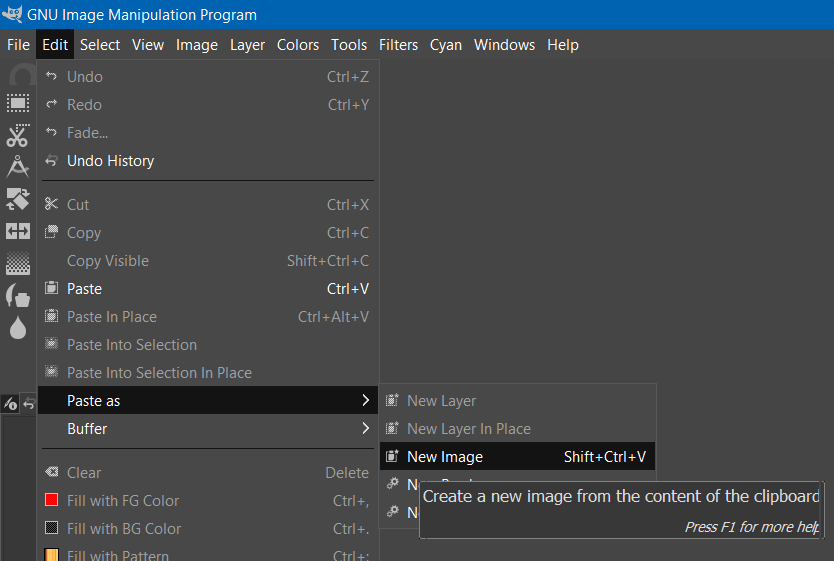
\includegraphics{images/screenshots/paste_as_new_gimp.png}

\begin{info}
Saving images with layers and text path information could come in handy
if you are generating your own image stimuli which features small
changes (such as different words), but remains mostly the same (same
background colour, size, fonts, etc).

In this case you could save a layer or export a different .GIF, .JPG or
.PNG from the same .XCF file for each change that you need to make.
\end{info}

\hypertarget{changing-image-size}{%
\paragraph{Changing Image Size}\label{changing-image-size}}
\addcontentsline{toc}{paragraph}{Changing Image Size}

Images that are too large can be resized in the \texttt{\textless{}img\textgreater{}} html tag to fit into a smaller space but if your image is too large you could be using more memory than would be required to store your images on the server.

This may have a knock on effect in the stimuli loading times.

Rather than consume excess bandwidth it is adviable to size the images down prior to uploading them on to the server.

To resize the image (and all layers and items contained within) click on the menu Image and press ``Scale Image\ldots{}''. This dialoue box will come up:

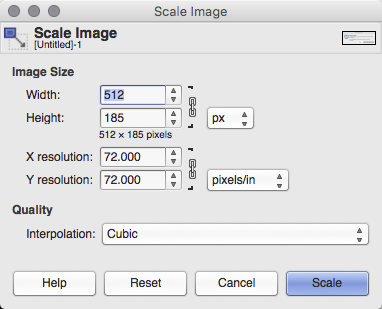
\includegraphics{images/screenshots/scale_image.png}

The image size defaults to \texttt{px}, or pixels. The height and the weight are by default linked together (as demonstrated by the chain symbol to the right of the two boxes). When linked changing either the height or the width will keep the image to the same aspect ratio (the proportions of the sizes). You may unlink the aspect ratio by clicking on the chain. When unlinked the chain will appear as broken.

Linking these helps you avoid distortion that might happen if you resize one dimension only, which might elongate/shorten the other dimension and make it look funny. It also allows you to make images to fit in a specific space in your study. For example, this word completion task where images are used instead of text:

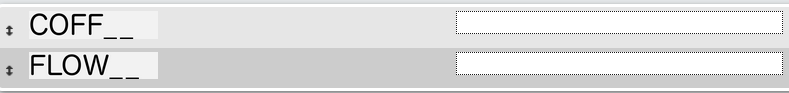
\includegraphics{images/screenshots/image_size_example.png}

I have used images in the question field of a mixed questionnaire, as the blank spaces are more apparent to the participants. I have also limited their size to 25px to ensure that they do not seem too oversized in comparison to the text entry fields next to them.

\hypertarget{exporting-images}{%
\paragraph{Exporting Images}\label{exporting-images}}
\addcontentsline{toc}{paragraph}{Exporting Images}

GIMP is capable of exporting GIF, JPEG and PNG file formats.

To export your image go to File \textgreater{} Export As. You will then be asked to enter a file name in the text box at the top of the dialogue box that opens up.

You can specify the type of file by typing the file extension at the end of the file name, ``.gif'', ``.jpg'' or ``.png'' for each of the aforementioned file types respectively.

Once you have done this, press the ``export'' button at the bottom of the dialogue box.

You may be asked to specify compression options after pressing the button. This is just to ask how much (if any) quality you are willing to sacrifice to save on the size of the file.

This is an example from a PNG file. This image was compressed with the default options. As you can tell the quality is good, but the image is not very rich. A richer image with higher levels of variation in the pixels may do worse that this one with the same level of compression.

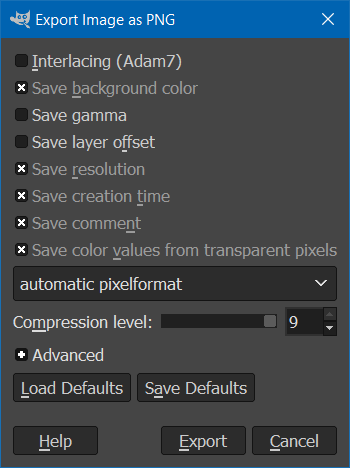
\includegraphics{images/screenshots/export_1.png}

When exporting JPEG files you will be asked to select the quality as a percentage, not compression level. The higher the percentage the higher the quality and the less compression being done.

Experiment with the levels of comrpression in the image and examine the outputs carefully for any artifacts in the images resulting from the compression process. If you find the quality lacking, lower the amount of compression allowed and try again until you find the level appropriate for your images.

These images are saved as JPEG, and are at 100\%, 50\% and 0\% quality. This gives file sizes of 76KB, 9KB and 2KB respectively:

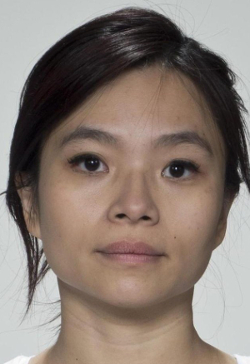
\includegraphics{images/screenshots/087_03_min.jpg}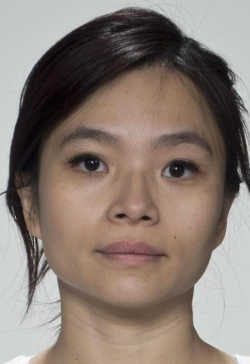
\includegraphics{images/screenshots/087_03_mid.jpg}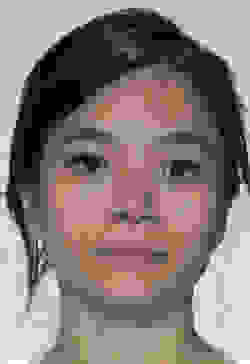
\includegraphics{images/screenshots/087_03_max.jpg}

The first is 100\% quality, no compression. The second has minimal pixelation artifacts around the periphery of the face, neck, hair and some issues with the skin texture in places. It also seems (to my office mates and I at least) that the skin tone is a ittle yellower in image 2. Number 3 is unusable.

\hypertarget{audio}{%
\subsection{Audio}\label{audio}}

Since Experimentum requires auditory stimuli to be uploaded as .mp3 files, here is an easy way to do batch processing.

\hypertarget{audacity-2.1.2}{%
\subsubsection{Audacity 2.1.2}\label{audacity-2.1.2}}

If you are still on an older version of audacity, go to \textbf{File -\textgreater{} Edit Chains}

There is already a chain set up for mp3 conversion, which contains 3 steps: Normalising, exporting as mp3, and an END process. You will probably have already normalised your stimuli, so highlight the first step of the chain and press delete.

All you should have in the chain ``MP3 Conversion'' is 1. ExportMP3, and 2. -END-. Click ``OK'' to save the chain.

Now, go to \textbf{File -\textgreater{} Apply Chain\ldots{}}

\ldots{} select MP3 Conversion, and confirm with ``Apply to Files''

Locate the files you want to have converted into MP3s from the folder on your computer, select all, and confirm with ``Open''.

The selected files will then be turned into mp3s. You will find an additional folder called ``cleaned'' within the folder your original files are located in.

Content of the folder ``cleaned'':

\hypertarget{audacity-2.3.0}{%
\subsubsection{Audacity 2.3.0}\label{audacity-2.3.0}}

For audacity version 2.3 and beyond, the batch-processing chains are now titled ``Macros'', and the menu got relocated to \textbf{Tools -\textgreater{} Macros\ldots{}}

Within the macros you will find one already labelled ``MP3 Conversion''. In the window ``Edit Steps'' (Num 01), select the normalise step and delete it.

Make sure you have only the steps ``ExportMP3'' and -END- left in your macro, the click on Files\ldots{}

\ldots{} and select the files you want to convert to mp3s. Highlight all of them and confirm with ``Open''.

There might be a warning message popping up asking you for an input method. Select the safer or faster option according to your personality, and confirm with ``OK''.

Once the process is done, you can find the converted mp3s in a separate folder called ``cleaned'' that is located within the folder of your original files.

\hypertarget{video}{%
\subsection{Video}\label{video}}

\hypertarget{uploading-stimuli}{%
\section{Uploading Stimuli}\label{uploading-stimuli}}

\hypertarget{using-stimuli}{%
\section{Using Stimuli}\label{using-stimuli}}

\hypertarget{assigning-stimuli-to-experimental-trials}{%
\subsection{Assigning Stimuli to Experimental Trials}\label{assigning-stimuli-to-experimental-trials}}

\hypertarget{using-stimuli-in-questionnaires}{%
\subsection{Using Stimuli in Questionnaires}\label{using-stimuli-in-questionnaires}}

\hypertarget{planning-your-project}{%
\chapter{Planning Your Project}\label{planning-your-project}}

\hypertarget{overview-2}{%
\section{Overview}\label{overview-2}}

\hypertarget{planning-your-project-1}{%
\section{Planning Your Project}\label{planning-your-project-1}}

\hypertarget{implementing-your-plan}{%
\section{Implementing Your Plan}\label{implementing-your-plan}}

\hypertarget{questionnaires}{%
\chapter{Questionnaires}\label{questionnaires}}

\hypertarget{overview-3}{%
\section{Overview}\label{overview-3}}

Questionnaires are currently the most used items on Experimentum. They are made up of one or more individual components, available in 3 different types: mixed, radiopage and ranking.

\hypertarget{new-questionnaire}{%
\section{New Questionnaire}\label{new-questionnaire}}

To create a new questionnaire, navigate to the researcher's section of the page by using the menu on the right and selecting the questionnaires option.


\includegraphics{images/screenshots/questionnaire_button.png}

From here, you will be able to see the questionnaires for which you have ownership status (ones you have created yourself, or ones that someone else has shared with you). To create a new questionnaire, click the button on the top right ``New Questionnaire'':

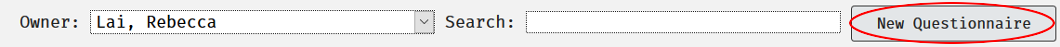
\includegraphics{images/screenshots/new_questionnaire.png}

The following pop-up box will appear, allowing you to choose the type that you want to create:

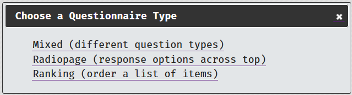
\includegraphics{images/screenshots/questionnaire_dialogue.png}

The types that you choose will depend on what type of functionality your study requires. You should note that pencil and paper questionnaires will not always be able to be copied exactly onto Experimentum. If you make any changes to questionnaires to deliver them electronically you should discuss required changes with your supervisor to ensure their validity has not been compromised.

\hypertarget{save-questionnaire-and-reset-buttons}{%
\section{Save Questionnaire and Reset Buttons}\label{save-questionnaire-and-reset-buttons}}

Once you have entered information about the questionnaire you should save it. Saving regularly is good practice. Do this by pressing the save questionnaire button.

The reset button is akin to a ``revert'' button, where any changes made after the last save can be discarded and you return to the last saved version.

\begin{danger}
The JavaScript for saving the questionnaire occasionally stops working
on some browsers, so we recommend saving the questionnaire after every 3
or so changes to minimise loss of work in the event of an error.

Please note that the site currently does not support version control, so
once you save a change the previous version will be overwritten.
\end{danger}

\hypertarget{questionnaires-information}{%
\section{Questionnaires Information}\label{questionnaires-information}}

All types of questionnaires will ask you to provide information about it, the only difference will be the Questionnaire Type, which will correspond to the type of questionnaire you have chosen on the previous pop-up box.

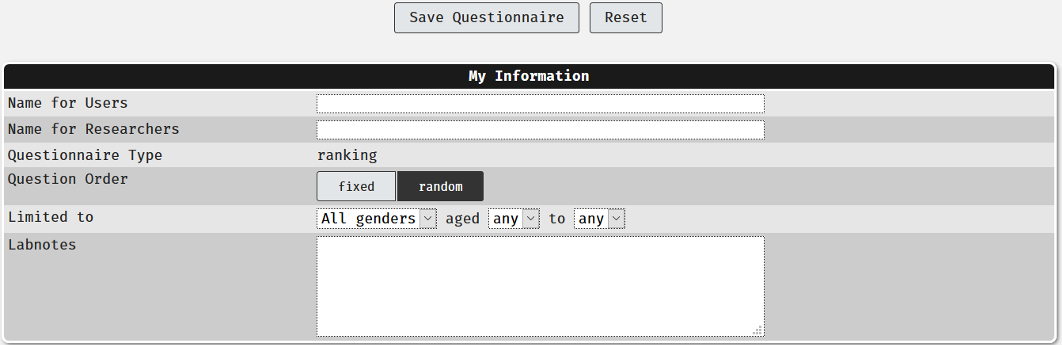
\includegraphics{images/screenshots/quest_info.png}

\begin{itemize}
\tightlist
\item
  \textbf{Name for Users}: this is the name of this component that will be displayed to users. Please ensure that it is appropriate.
\item
  \textbf{Name for Researchers}: this is the name of this component for researchers. It will be displayed on lists and visible to you, your supervisor and admin staff. It should be informative and appropriate.
\item
  \textbf{Question Order}: this indicates how you want Experimentum to display the questions contained \textbf{in this component only}.

  \begin{itemize}
  \tightlist
  \item
    Fixed will display the questions to the participants in the order you have put them on this page.
  \item
    Random will mix the order of question presentation up automatically. Order of presentation will be recorded in your data when you download it.
  \end{itemize}
\item
  \textbf{Limited to}: limitations will only allow people in a certain age range and with a certain gender identity to complete this component of the study.

  \begin{itemize}
  \tightlist
  \item
    If you are planning on allowing anonymous participation you should not set limitations as age and gender identity of these users will be unknown and may not be allowed to do these sections of the study if participants refuse this information.
  \end{itemize}
\item
  \textbf{Labnotes}: this is a short blurb about this component of your study. You should always add lab notes so that you, your supervisor and the admins will be able to tell what this component is about.
  The following sections will describe each questionnaire type and what they can do.
\end{itemize}

\hypertarget{questionnaire-tab}{%
\section{Questionnaire Tab}\label{questionnaire-tab}}

The questionnaire tab on the lower half of the page is different for each questionnaire. Please see the appropriate sections below for more information on these.

\hypertarget{feedback-tab}{%
\section{Feedback Tab}\label{feedback-tab}}

In most cases you should leave this empty. The feedback for the top-most set is normally where you would put your debriefing information. You can see the later sections on projects and debriefing.

\hypertarget{adding-and-deleting-questions}{%
\section{Adding and Deleting questions}\label{adding-and-deleting-questions}}

\hypertarget{adding-individually}{%
\subsection{Adding Individually}\label{adding-individually}}

In order to add a new question, you must ensure that all editing options are closed on the existing questions by clicking the pencil to get rid of the yellow surround or the cog to close the menu.
Pressing the button at the bottom of the page will allow you to add a new question.

Experimentum will add a new question by directly duplicating the previous question, with all the same text and attributes. Please ensure that you set a unique name for the new question before you attempt to save the questionnaire as questions with duplicate names will be removed by the system.

\begin{danger}
The JavaScript for saving the questionnaire occasionally stops working
on some browsers, so we recommend saving the questionnaire after every 3
or so changes to minimise loss of work in the event of an error.
\end{danger}

\hypertarget{adding-in-bulk}{%
\subsection{Adding in Bulk}\label{adding-in-bulk}}

It is also possible to add some types of questions in bulk by using a spreadsheet. Unfortunately, not all types are covered, but the most basic and most frequently used types are.
Spreadsheet templates are available by clicking ``add from spreadsheet'' and selecting the underlined type of questionnaire from the options just above the buttons.

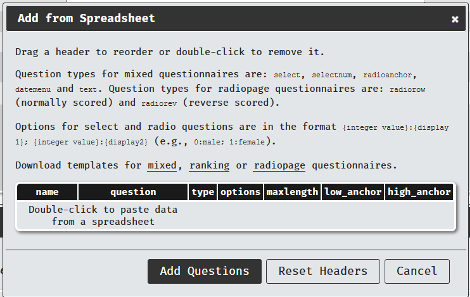
\includegraphics{images/screenshots/quest_spread_1.png}

Each of the column headers will relate to each of the question attributes you would use when setting the questions manually. For ranking and radiopage questionnaires not all of these headers will be applicable. Double click on the ones you do not need to remove them as I have done in the image below:

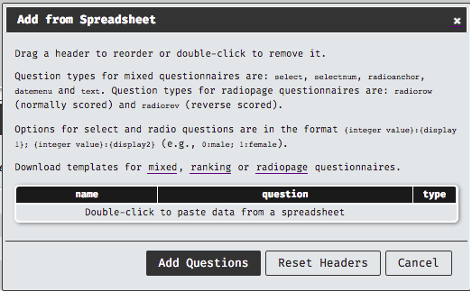
\includegraphics{images/screenshots/quest_spread_2.png}

Fill the template spreadsheet in and save it onto your own storage, copy the cells that contain your question information. See the section below for more about question information.
Double click on the section that says, ``Double-click to paste data from a spreadsheet'' and paste it when in the new entry box that appears:

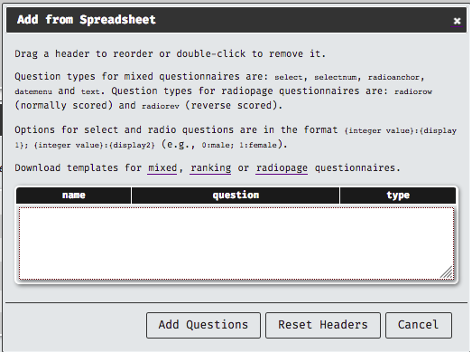
\includegraphics{images/screenshots/quest_spread_3.png}

If you do not use the template spreadsheet, but one you have made yourself, ensure that the options that you are specifying match. You can also drag the headers on the entry window from left to right to re-order them if your own spreadsheet does not match the headers here.

\begin{tabular}{l|l|l}
\hline
Column Header: & Refers to: & Options:\\
\hline
name & dv\_name (in data = q\_name) & Names must only contain letters, underscores and numbers (numbers must not be the first characters).\\
\hline
question & The question that you are asking the participant. & Whatever you want to ask the participant.\\
\hline
type & The type of question, akin to the options selected from the menu opened by the cog & * select: pulldown menu \textbackslash{}n* selectnum: numeric pulldown menu \textbackslash{}n* radio: radiobuttons \textbackslash{}n* radioanchor: radiobuttons with anchors \textbackslash{}n* datemenu: date menu \textbackslash{}n* text: short text\\
\hline
options & Where you would specify the response options available to the participants. & Applicable to select and radio types. \textbackslash{}n*  Numerical code, followed by ":", and then text option. \textbackslash{}n*  Specifying multiple by separating options using a semi-colon (;)\\
\hline
maxlength & Where you would specify the length of the response & Applicable to radioanchor and text. \textbackslash{}n*  Radioanchor: how many points in the range. \textbackslash{}n*  Text: how many characters allowed.\\
\hline
low\_anchor & Specifying the low anchor for the selected option. & Applicable to selectnum, radioanchor and datemenu. \textbackslash{}n*  Selectnum specifies the lowest number in the range of the dropdown menu \textbackslash{}n*  Radioanchor specifies the text for low anchor \textbackslash{}n*  Datemenu specified the lower end of the year range.\\
\hline
high\_anchor & Specifying the high anchor for the selected option. & Applicable to selectnum, radioanchor and datemenu. \textbackslash{}n*  Selectnum specifies the highest number in the range of the dropdown menu\textbackslash{}n*  Radioanchor specifies the text for high anchor\textbackslash{}n*  Datemenu specified the higher end of the year range.\\
\hline
\end{tabular}

\hypertarget{deleting-questions}{%
\subsection{Deleting Questions}\label{deleting-questions}}

Questions can be erased by clicking the picture of the trash/bin next to the question you want to delete.


\includegraphics{images/screenshots/bin.png}

\begin{danger}
Please note that the site currently does not support version control, so
once you save a change the previous version will be overwritten. This
includes deleted questions- once you have saved the changes they are
gone.
\end{danger}

\hypertarget{questionnaire-types}{%
\section{Questionnaire Types}\label{questionnaire-types}}

\hypertarget{mixed-questionnaire}{%
\subsection{Mixed Questionnaire}\label{mixed-questionnaire}}

Allows you to present multiple question types and gather multiple response types in a single component. When you select a mixed questionnaire, you will be taken to this page:

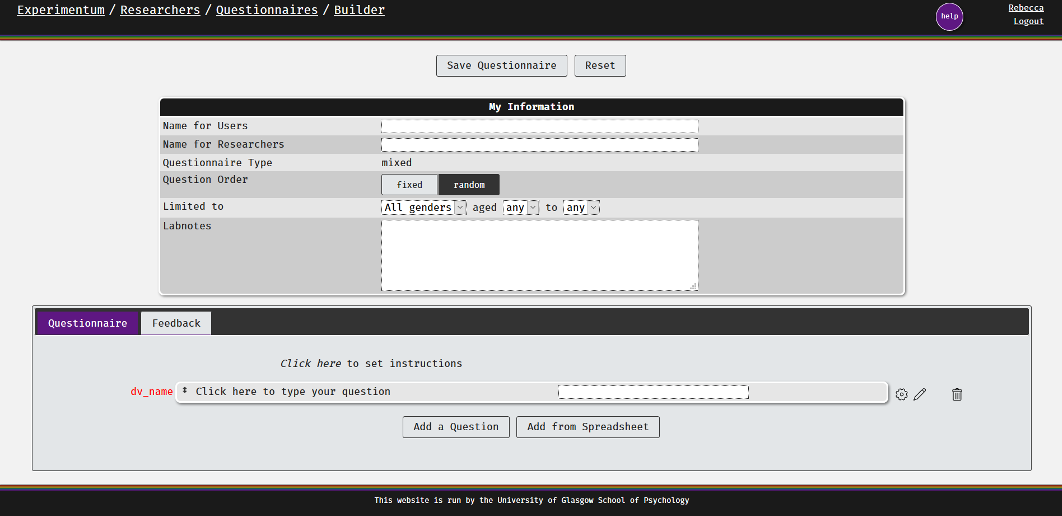
\includegraphics{images/screenshots/quest_mixed.png}

As you can see you have the same questionnaire information section at the top, as you will have in all questionnaires. The differences lie in the types of questions that you can include. Mixed questionnaires can accommodate multiple types of questions on a single page.

\begin{itemize}
\tightlist
\item
  \textbf{Instructions}: when you click the part that says ``Click here to set instructions'' you will be able to enter text instructions to the participants for this entire component. You will also be able to enter Markdown and HTML code, which allows you to link to and embed additional media or format the text in specific ways.

  \begin{itemize}
  \tightlist
  \item
    If you use HTML tags you must ensure that you have matching opening and closing tags, as unmatched ones will prevent the component from recording data.
  \end{itemize}
\item
  \textbf{dv\_name}: this is the name of the dependent variable, the name that will be assigned to the column q\_name in the downloaded data indicating which question the participant has answered. You should set one which is unique to this component and perhaps across all components.
\item
  \textbf{Question}: clicking the part which says ``click here to set your question'' will allow you to enter the question text that the participants will see, the question that you want to ask them.
\end{itemize}

\hypertarget{changing-question-and-response-type}{%
\subsubsection{Changing Question and Response Type}\label{changing-question-and-response-type}}

Clicking the cog next to the question and then the arrow in the resulting menu will allow you to choose the type of question you want to set.

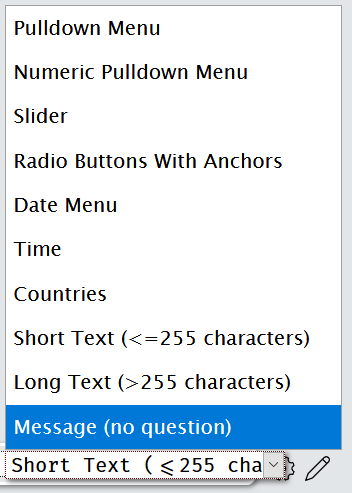
\includegraphics{images/screenshots/quest_mixed_1.png}

When you have selected the type of question, you can then edit the response types that can be made by the participants by clicking the pencil next to the cog. When this editing mode is active, the response section will be unfolded, and will be displayed with a yellow surround.

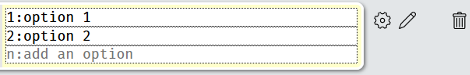
\includegraphics{images/screenshots/quest_mixed_2.png}

\begin{warning}
You must close this editing mode by clicking the pencil a second time,
getting rid of the yellow surround, \textbf{before} you add a new
question, click the cog or save the questionnaire.
\end{warning}

In the section below I will cover the types of questions and information about the changes to the participant responses in the appropriate sections below.

\begin{itemize}
\tightlist
\item
  \textbf{Pulldown Menu}: pulldown menus give your participants a set of text option responses to choose from. Each text option has a numeric coding value associated with it, which will be the returned value in the downloaded data in place of the text. This is specified before the colon. The text options are specified after the colon, these are not returned in the data.

  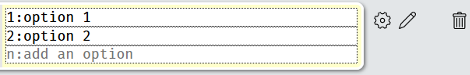
\includegraphics{images/screenshots/quest_mixed_3.png}

  \begin{itemize}
  \tightlist
  \item
    Each text value should be associated with a unique numerical coding value, non-unique numerical codes will be deleted upon saving the questionnaire. You can add multiple options to the menu.
  \end{itemize}
\item
  \textbf{Numeric Pulldown Menu}: this allows you to set numerical values to a pulldown menu, with no associated text label. The range that is set is the range that will be displayed to the user, as below.

  \begin{itemize}
  \tightlist
  \item
    You should use whole numbers only.

    
\includegraphics{images/screenshots/quest_mixed_4.png}

    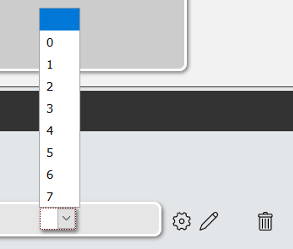
\includegraphics{images/screenshots/quest_mixed_5.png}
  \end{itemize}
\item
  \textbf{Slider}: sliders provide you with a way for participants to return a finer-grained numerical response on a spectrum between two anchor points. A slider scale will be displayed to participants, with the low end of the range associated with the low anchor, and the high end the high anchor. Participants will move a slider along the scale, and a numerical value associated with the position they put it in returned in the data. You set the scale limits and increments, in this example from 0 to 100 in increments of 1.

  \begin{itemize}
  \tightlist
  \item
    You can also change the text anchors by clicking on them as shown here.

    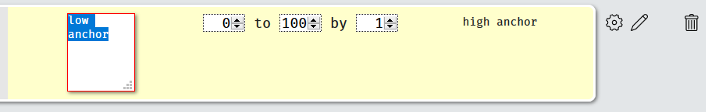
\includegraphics{images/screenshots/quest_mixed_6.png}
  \end{itemize}
\item
  \textbf{Radio Buttons with Anchors}: this option allows you to set a scale with a low anchor and a high anchor, which you can change by clicking the text. You can add or remove points to the scale by pressing the + and -- buttons on either side of the response. On this scale example below, a number will be returned associated with the point on the scale the participant submitted, here 1 (lowest) to 5 (highest).

  
\includegraphics{images/screenshots/quest_mixed_7.png}
\item
  \textbf{Date Menu}: date menus allow the participants to choose a specific date. You can set the range of dates to choose from, in the example below the participant is allowed to go back 100 years from the current date (-100y) but cannot go further into the future than today (+0y). When participants click on the response, they will be given a calendar to pick from, instead of typing the date.

  
\includegraphics{images/screenshots/quest_mixed_8.png}

  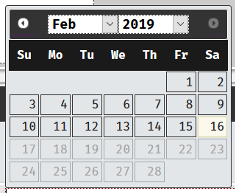
\includegraphics{images/screenshots/quest_mixed_9.png}
\item
  \textbf{Countries}: participants can choose from a list countries. Returned in the data as the two letter ISO-3166-1 code.

  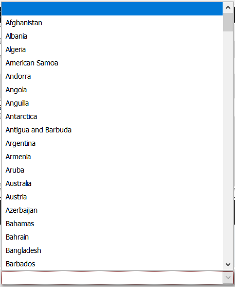
\includegraphics{images/screenshots/quest_mixed_10.png}
\item
  \textbf{Short Text}: allows participants to enter free-response text up to and including 255 characters. Returned in the data as character strings.

  
\includegraphics{images/screenshots/quest_mixed_11.png}
\item
  \textbf{Long Text}: allows participants to enter free-response text over 255 characters. Returned in the data as character strings. If you do not need more than 255 characters, please use the short text to minimise strain on the server.

  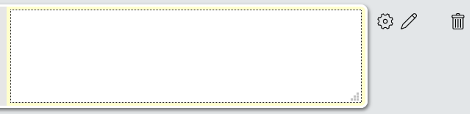
\includegraphics{images/screenshots/quest_mixed_12.png}
\end{itemize}

\hypertarget{experimental-components}{%
\chapter{Experimental Components}\label{experimental-components}}

\hypertarget{overview-4}{%
\section{Overview}\label{overview-4}}

\hypertarget{sets}{%
\chapter{Sets}\label{sets}}

\hypertarget{overview-5}{%
\section{Overview}\label{overview-5}}

\hypertarget{projects}{%
\chapter{Projects}\label{projects}}

\hypertarget{overview-6}{%
\section{Overview}\label{overview-6}}

\hypertarget{project-urls}{%
\section{Project URLs}\label{project-urls}}

\hypertarget{anon}{%
\section{Anonymous Participation}\label{anon}}

\hypertarget{knownissues}{%
\chapter*{Known Issues and Bugs}\label{knownissues}}
\addcontentsline{toc}{chapter}{Known Issues and Bugs}

\hypertarget{overview-7}{%
\section*{Overview}\label{overview-7}}
\addcontentsline{toc}{section}{Overview}

This is a list of issues that are known and that we are working on to fix.

If you discover another issue that is not listed here you can report the issue \href{https://github.com/RebeccaJLai/exp_manual/issues}{here}- but please check that it has not been reported before you open another issue for it.

\hypertarget{issues}{%
\section*{Issues\ldots{}}\label{issues}}
\addcontentsline{toc}{section}{Issues\ldots{}}

\hypertarget{which-do-not-interfere-with-the-operation-of-the-site}{%
\subsection*{Which do NOT interfere with the operation of the site}\label{which-do-not-interfere-with-the-operation-of-the-site}}
\addcontentsline{toc}{subsection}{Which do NOT interfere with the operation of the site}

These issues are bugs which do not prevent the intended function of the action being carried out at the time of their occurrance and are considered to be of low priority.

\hypertarget{notfound}{%
\subsubsection*{``The supervisor or supervised could not be found'' when changing account type}\label{notfound}}
\addcontentsline{toc}{subsubsection}{``The supervisor or supervised could not be found'' when changing account type}

This happens when a supervisor attempts to change the account type of a student from ``registered'' to ``student''. The account changes are carried out regardless of the message.

To check this log out, log back in and then check the status of the student.

\begin{info}
The account being changed must log out and then back in for any changes
to take effect, regardless of whether you experience this bug or not.
\end{info}

\hypertarget{which-do-interfere-with-the-operation-of-the-site}{%
\subsection*{Which DO interfere with the operation of the site}\label{which-do-interfere-with-the-operation-of-the-site}}
\addcontentsline{toc}{subsection}{Which DO interfere with the operation of the site}

These issues are bugs which in some way inhibit the function of the site and are considered high priority for fixes and workarounds.

\hypertarget{email-notifications}{%
\subsubsection*{Email Notifications}\label{email-notifications}}
\addcontentsline{toc}{subsubsection}{Email Notifications}

Email notifications are not always sent.

E-mails notifying students and supervisors of changes of account type work seemingly without issue. In particular, e-mails requesting supervisors turn studies to ``active'' are not being sent.

\begin{workaround}
\textbf{Workaround:} Please e-mail your supervisor directly if you
require them to review and activate your study.
\end{workaround}

\hypertarget{cannot-share-ownership-of-components-with-students}{%
\subsubsection*{Cannot Share Ownership of Components With Students}\label{cannot-share-ownership-of-components-with-students}}
\addcontentsline{toc}{subsubsection}{Cannot Share Ownership of Components With Students}

At the moment it is not possible to share components with students. This stems from a work-around regarding access to and protection of data. Anyone who is an owner of a component may download the data gathered by it, even if that component is also used by others.

\begin{workaround}
\textbf{Workaround:} At the moment it is recommended that students
create their own components to suit their needs or that the supervisor
duplicate the component and assign the duplicate to the student in need.

If the supervisor is making a component specifically for that student
and no-one else will or should have access to that data contact an admin
on the Slack workspace for another workaround that only they have the
ability to implement.
\end{workaround}

\hypertarget{faqs}{%
\chapter*{FAQs}\label{faqs}}
\addcontentsline{toc}{chapter}{FAQs}

\hypertarget{overview-8}{%
\section*{Overview}\label{overview-8}}
\addcontentsline{toc}{section}{Overview}

The most commonly asked questions, documented here so that you can review the potential solutions.

Potential workaround for common bugs awaiting a fix are documented in the \protect\hyperlink{knownissues}{Known Issues} chapter.

\hypertarget{about-support}{%
\section*{About Support}\label{about-support}}
\addcontentsline{toc}{section}{About Support}

\hypertarget{i-emailed-an-admin-and-havent-received-a-response}{%
\subsection*{I emailed an admin and haven't received a response}\label{i-emailed-an-admin-and-havent-received-a-response}}
\addcontentsline{toc}{subsection}{I emailed an admin and haven't received a response}

In addition to helping you with Experimentum we also have our own research and teaching responsibilities. As a result, our inboxes are usually very full, and emails will inevitably be missed. All students and staff should use the appropriate ``Experimentum-web'' slack workspace channel if they have support issues as this is the most reliable method of contact.

\hypertarget{about-accounts}{%
\section*{About Accounts}\label{about-accounts}}
\addcontentsline{toc}{section}{About Accounts}

\hypertarget{i-have-requested-researcher-status-and-havent-received-it}{%
\subsection*{I have requested researcher status and haven't received it}\label{i-have-requested-researcher-status-and-havent-received-it}}
\addcontentsline{toc}{subsection}{I have requested researcher status and haven't received it}

Your supervisor is the person responsible for upgrading your account with the appropriate permissions.

Admins are not responsible for tracking who is entitled to what access levels.

If your supervisor is experiencing technical difficulties in changing your status it is their responsibility to report these issues to the admins, not yours. No third party request on behalf of a supervisor to change access levels will be accepted by admins.

Members of teaching staff who are supervising students and experiencing delay in receiving appropriate permissions should contact Professor DeBruine or Rebecca as a matter of urgency via direct message on the appropriate Slack workspace.

Researcher status will not be granted to students, researchers or members of the public who do not have an official role at the University of Glasgow School of Psychology.

\hypertarget{my-supervisor-approved-my-researcher-status-but-my-account-doesnt-have-updated-privileges}{%
\subsection*{My supervisor approved my researcher status, but my account doesn't have updated privileges}\label{my-supervisor-approved-my-researcher-status-but-my-account-doesnt-have-updated-privileges}}
\addcontentsline{toc}{subsection}{My supervisor approved my researcher status, but my account doesn't have updated privileges}

If you are logged in when your supervisor makes these changes you will need to log out and back in again for your privileges to be updated correctly. If this does not resolve the issue contact the admins for support.

\hypertarget{i-have-lost-my-password}{%
\subsection*{I have lost my password}\label{i-have-lost-my-password}}
\addcontentsline{toc}{subsection}{I have lost my password}

Automated password retrieval is not an option. All account holders can request a new, temporary password by contacting an admin or their supervisor.

Supervisors and researchers may also issue temporary passwords to their students and participants but should ensure that they take all necessary measures to verify their identity and right to access the account. This could be through the production of student or other photographic ID. If their identity cannot be verified the password should not be reset and instead they should be asked to register for a new account.

All temporary passwords should be changed as soon as possible through the Account options on Experimentum.

\hypertarget{about-study-constructionactivation}{%
\section*{About Study Construction/Activation}\label{about-study-constructionactivation}}
\addcontentsline{toc}{section}{About Study Construction/Activation}

\hypertarget{my-questionnaireresponses-to-questions-wont-save}{%
\subsection*{My questionnaire/responses to questions won't save}\label{my-questionnaireresponses-to-questions-wont-save}}
\addcontentsline{toc}{subsection}{My questionnaire/responses to questions won't save}

Occasionally the JavaScript that allows you to save changes you have made to your questionnaire will stop working, meaning that you will lose those changes. You should save your questionnaires regularly to ensure that if this happens you won't lose too much work. I recommend saving after every 2-3 questions.

Codes assigned to response variables should be unique within that question, otherwise they will overwrite each other, and duplicate options will be removed.

Editing options for responses to questions must be closed before you attempt to save the questionnaire by re-clicking the pencil icon next to the cog. You can tell that editing is open by the yellow colour surrounding the response options as below.

\hypertarget{can-the-system-make-studies-which-branch-depending-on-the-responses-given-by-participants}{%
\subsection*{Can the system make studies which branch depending on the responses given by participants?}\label{can-the-system-make-studies-which-branch-depending-on-the-responses-given-by-participants}}
\addcontentsline{toc}{subsection}{Can the system make studies which branch depending on the responses given by participants?}

This is currently an extremely limited option. It is possible to allow participants to self-select a set by placing multiple sets within a project. Participants will then complete the set that they have selected.

Unfortunately, it is not possible to filter participants to specific components based upon their responses to questionnaires or experiments (i.e.~screening, where you would want participants to complete the Beck Depression Inventory (Beck et al., 1988) or the Autism Spectrum Quotient, 10-item (Booth et al., 2013) and having only those who meet a certain threshold complete further components).

\hypertarget{i-edited-my-study-and-it-changed-from-active-to-test.-how-do-i-change-it-back}{%
\subsection*{I edited my study and it changed from active to test. How do I change it back?}\label{i-edited-my-study-and-it-changed-from-active-to-test.-how-do-i-change-it-back}}
\addcontentsline{toc}{subsection}{I edited my study and it changed from active to test. How do I change it back?}

Supervisors are responsible for making sure that your student project is suitably constructed and are the only ones who can authorise you to start collecting data.

When you make any change to your study, Experimentum will change the status back to test automatically. Changes must be approved by your supervisor to ensure they have not invalidated your study. When they are satisfied that your study meets the standard that they expect, and that the changes are appropriate, they can change the study back to active for you.

You should be aware that changes to your study may render the data collected prior to the changes incomparable with data collected after. Changes should not be made after projects have been set to active unless a) the changes are minimal (for example, correcting a typo) or b) where you are willing to accept the possibility that your data prior to/after the change could potentially be invalidated.

It is not the job of the admins to approve changes to your study, as we are not likely to have adequate knowledge of your specialisation to assess it meets the appropriate standard. If your supervisor experiences technical issues in doing this then they must contact admins via the appropriate Slack workspace.

\hypertarget{my-studycomponents-of-my-study-are-set-to-test.-how-do-i-make-it-active}{%
\subsection*{My study/components of my study are set to test. How do I make it active?}\label{my-studycomponents-of-my-study-are-set-to-test.-how-do-i-make-it-active}}
\addcontentsline{toc}{subsection}{My study/components of my study are set to test. How do I make it active?}

Your supervisor is the person responsible for making this change from test to active when they are satisfied that it meets the standard that they expect.

As we do not have expertise in your specialisation, we cannot assess that it meets the appropriate standard. If your supervisor is experiencing technical issues in attempting to do this it is their responsibility to contact the admins, not yours.

\hypertarget{where-do-i-put-my-informationdebrief-sheet}{%
\subsection*{Where do I put my information/debrief sheet?}\label{where-do-i-put-my-informationdebrief-sheet}}
\addcontentsline{toc}{subsection}{Where do I put my information/debrief sheet?}

Your information sheet should usually be entered on the introduction section of the project page. The debrief sheet, likewise, should usually be entered into the feedback section of the top-most set within the project.

See the diagrams at the ``Debriefing'' section of this document.

In certain circumstances it might be put elsewhere, such as when your participants complete different study components. If you do not know where to put your debrief, seek support.

\hypertarget{can-i-have-multiple-response-scales-on-a-single-radiopage-questionnaire}{%
\subsection*{Can I have multiple response scales on a single radiopage questionnaire?}\label{can-i-have-multiple-response-scales-on-a-single-radiopage-questionnaire}}
\addcontentsline{toc}{subsection}{Can I have multiple response scales on a single radiopage questionnaire?}

Unfortunately, this cannot currently be done. Consider making a radio page per scale and combining them into a set.

This is most commonly asked in relation to the next question, ``Does my Experimentum questionnaire need to look exactly like the paper version?''.

\hypertarget{does-my-experimentum-questionnaire-need-to-look-exactly-like-the-paper-version}{%
\subsection*{Does my Experimentum questionnaire need to look exactly like the paper version?}\label{does-my-experimentum-questionnaire-need-to-look-exactly-like-the-paper-version}}
\addcontentsline{toc}{subsection}{Does my Experimentum questionnaire need to look exactly like the paper version?}

Not always. Paper questionnaires were limited by issues like available printing resources and ease of data input. With electronic delivery this is no longer a concern, and the system can delivery added utility such as question randomisation.

If you are concerned that changing the presentation of the instrument you are using has impacted its validity you should discuss these concerns with your supervisors.

\hypertarget{about-study-participation}{%
\section*{About Study Participation}\label{about-study-participation}}
\addcontentsline{toc}{section}{About Study Participation}

\hypertarget{my-participants-are-not-being-allowed-to-take-part-in-my-studya-part-of-my-study}{%
\subsection*{My participants are not being allowed to take part in my study/a part of my study}\label{my-participants-are-not-being-allowed-to-take-part-in-my-studya-part-of-my-study}}
\addcontentsline{toc}{subsection}{My participants are not being allowed to take part in my study/a part of my study}

This usually happens when you allow anonymous participation but have chosen to set limitations on gender identity and age range on a component, set or project.

Anonymous users ages and genders are not known, thus their eligibility to take part on studies with limitations is not able to be assessed. It used to be that the system would pass the participants directly past the parts of the study with limitations.

As a way to combat this, participants of anonymous studies will now see a dialogue box asking for their age and gender identity. If the participants fill in this information and they meet the requirements they will see your study as normal. If they refuse this information they will still bypass the parts of the study with limitations as we cannot tell if they are eligible to participate.

If you wish to gather information from participants then you must always respect their right not to answer all of your questions, including their age and gender identity. If this information is refused, then they may not be able to take part in your study.

We recommend that if you do not have a strong theoretical or ethical reason to limit participation by these characteristics then you do not place limitations on any part of your study.

\hypertarget{about-data}{%
\section*{About Data}\label{about-data}}
\addcontentsline{toc}{section}{About Data}

\hypertarget{missing-data}{%
\subsection*{Missing Data}\label{missing-data}}
\addcontentsline{toc}{subsection}{Missing Data}

Truly missing data is rare. Data can be misattributed to a different study if participants are completing more than one study at the same time. Therefore, we recommend that you download your data from each of the individual components from your study rather than downloading the data from the entire project page- see ``Downloading Your Data''.

All data recorded under the individual components will be contained in the CSV file, regardless of what project it has been attributed to.

You should also bear in mind that online studies are particularly prone to attrition, especially if they are longer in duration. If you have concerns about missing data, contact the admins for support.

\hypertarget{where-is-my-data-stored}{%
\subsection*{Where is my data stored?}\label{where-is-my-data-stored}}
\addcontentsline{toc}{subsection}{Where is my data stored?}

Your data is stored on site at the University of Glasgow School of Psychology.

\hypertarget{supervisor-cheatsheet}{%
\chapter*{Supervisor Cheatsheet}\label{supervisor-cheatsheet}}
\addcontentsline{toc}{chapter}{Supervisor Cheatsheet}

\hypertarget{overview-9}{%
\section*{Overview}\label{overview-9}}
\addcontentsline{toc}{section}{Overview}

This is a collection of sections from the document directed at the everyday operations that supervisors would need to carry out assembled in one place for easy reference.

If there is anything missing please file an issue on the GitHub codebase for this book by clicking \href{https://github.com/RebeccaJLai/exp_manual/issues}{here}.

\hypertarget{roles}{%
\section*{Admins}\label{roles}}
\addcontentsline{toc}{section}{Admins}

Lisa is busy and Rebecca is contracted for 1 hour per week for Experimentum support. Much of the day-to-day of handling your students will fall on you, the supervisor.

If you are not prepared to accept this you may need to consider using another system.

\hypertarget{admin-responsibilities}{%
\subsection*{Admin Responsibilities}\label{admin-responsibilities}}
\addcontentsline{toc}{subsection}{Admin Responsibilities}

Our responsibilities are:

\begin{itemize}
\tightlist
\item
  To try to ensure smooth operation of the site with regards to technical difficulties and instruction of staff and students.

  \begin{itemize}
  \tightlist
  \item
    We will hold workshops at specific time points throughout the academic year, update this manual and answer questions on Slack.
  \end{itemize}
\item
  To troubleshoot problematic issues experienced by staff and students.
\end{itemize}

\hypertarget{supervisor-responsibilities}{%
\subsection*{Supervisor Responsibilities}\label{supervisor-responsibilities}}
\addcontentsline{toc}{subsection}{Supervisor Responsibilities}

\begin{itemize}
\tightlist
\item
  To ensure that you have a researcher account to supervise any of your students who wish to use the site.

  \begin{itemize}
  \tightlist
  \item
    You may be comfortable allowing some more senior and trustworthy students almost complete autonomy by granting them full researcher status but it is still advisable to have an account of your own.
    \textbf{\emph{If you wish for them to have full researcher status this must be confirmed by the supervisor to Rebecca directly, not through your student or third party.}}
  \end{itemize}
\item
  To handle the day-to-day needs of your own students:

  \begin{itemize}
  \tightlist
  \item
    Ensure that you have the knowledge to know how to implement designs you expect your students to use through the site.
  \item
    To check the standards of your students work.
  \item
    To approve ``student'' researcher status of your own students.
  \item
    To activate the projects of your own students, even when they deactivate them by making edits after an initial activation.
  \item
    To manage your students expectations of what the site can provide (it will not be perfect or even workable for some types of study).
  \end{itemize}
\end{itemize}

\begin{warning}
Supervisors should supervise their own students' accounts only, unless
they have the expertise to double-check the veracity of the students'
work and are prepared to accept the responsibilities outlined above for
these students.
\end{warning}

\hypertarget{approving-student-and-researcher-status-requests-1}{%
\section*{Approving Student and Researcher Status Requests}\label{approving-student-and-researcher-status-requests-1}}
\addcontentsline{toc}{section}{Approving Student and Researcher Status Requests}

Supervisors have a responsibility to ensure that their students have the status that they require to carry out their projects. This includes assigning them sufficient permissions to construct and deploy their studies.

Once the supervisor has ``researcher'' status they will have a new area of the website opened to them, accessible through the researchers' link in the menu on the right, which will contain a section called ``Admin'':

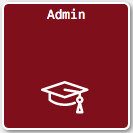
\includegraphics{images/screenshots/admin_button.png}

Clicking on this button will take them to a page with more options. To see and make changes to the privileges of those who have requested you as a supervisor and requested researcher status select the option ``Supervision'' from the menu.

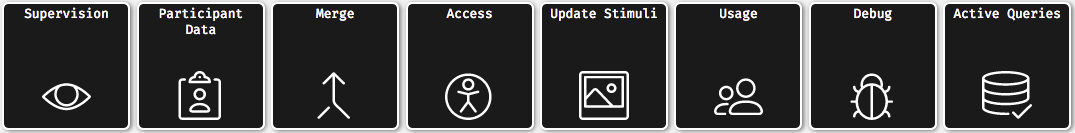
\includegraphics{images/screenshots/admin_options.png}

Here you will see a list of individuals who have requested you as a supervisor. To change their status, select the appropriate account type from the right-most drop-down menu under the column ``Status''.


\includegraphics{images/screenshots/status_bar.png}

The account you are making changes to will have to log out and back in again to be updated with their new permissions. When you press ``Send'' an email will be sent to the student to inform them of the status change.

\begin{info}
If you are a supervising member of teaching or research staff, you
should request Lisa DeBruine or Rebecca Lai as your supervisor.

More senior students who are relatively self-sufficient or have their
own supervising duties may request ``researcher'' accounts \emph{if you,
their supervisor, agrees to it and contacts Rebecca about it directly}.
No such request will be accepted on the word of a student or request via
third party.

In such a case where this is agreed they should request Lisa or Rebecca
as their supervisor as any other ``researcher'' account would.
\end{info}

\hypertarget{activating-studies}{%
\section*{Activating Studies}\label{activating-studies}}
\addcontentsline{toc}{section}{Activating Studies}

\begin{warning}
Once you activate a study for a ``student'' researcher account it cannot
be edited without resetting it back to ``test'' status, essentially
deactivating it.

Students should confirm that they are completely happy with the study
before they ask you to activate it.

If a student makes a change to the study after activation, rendering it
inactive, you the supervisor are the point of contact for the student to
reactivate it. You may wish to check that the edits made have not
changed the quality of the project.
\end{warning}

\hypertarget{resetting-passwords}{%
\section*{Resetting Passwords}\label{resetting-passwords}}
\addcontentsline{toc}{section}{Resetting Passwords}

Researcher status accounts also have permission to reset some passwords, found by searching in the ``Participant Data'' section in the admin page, but they should limit this to resetting the passwords of their own students or participants.

\begin{danger}
You must be satisfied that the account holder is the person requesting
the change of password.

In terms of students conducting research projects I would recommend that
they present themselves to you in person to request a password change as
these students have access to participant data.
\end{danger}

To change a password, you can either:

\begin{itemize}
\item
  Navigate to Researchers, then Admin and finally to Participants and search for either the entire or partial username or ID number and click ``reset password'' \textbf{or}
\item
  Find your student under your supervisory list by going to Researchers, then Admin, then Supervision and selecting their name from the list and selecting ``reset password.
\end{itemize}

The new password will be displayed on the page straight away on the page:

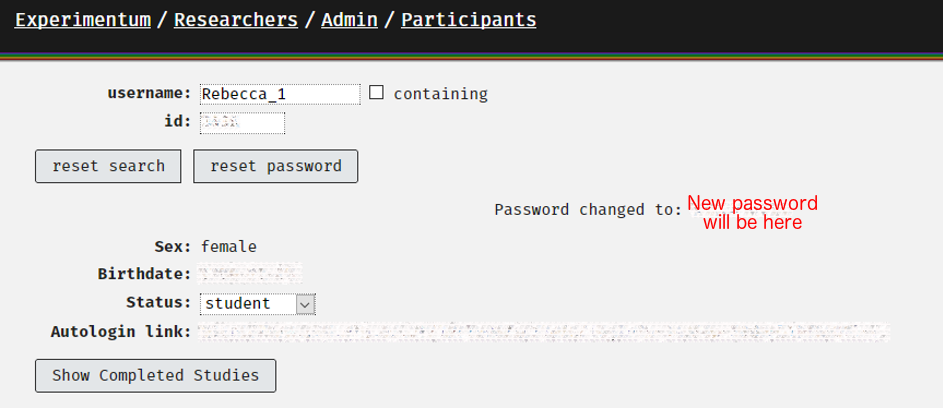
\includegraphics{images/screenshots/reset_password.png}

\begin{danger}
This password is supposed to be temporary, but it does not expire. It
should be changed as soon as possible as it will have likely be
communicated via e-mail or will have been written down.
\end{danger}

\hypertarget{autologin-links}{%
\section*{Autologin Links}\label{autologin-links}}
\addcontentsline{toc}{section}{Autologin Links}

Autologin links allow you to by-pass password verification and access the accounts of those that you supervise. These exist to allow admins and supervisors to log in to student's accounts to examine their studies and help when required.

You can access your student's autologin link by navigating to ``Researchers'' \textgreater{} ``Admin'' \textgreater{} ``Supervision'' and clicking on the student's name from your list of supervisees:

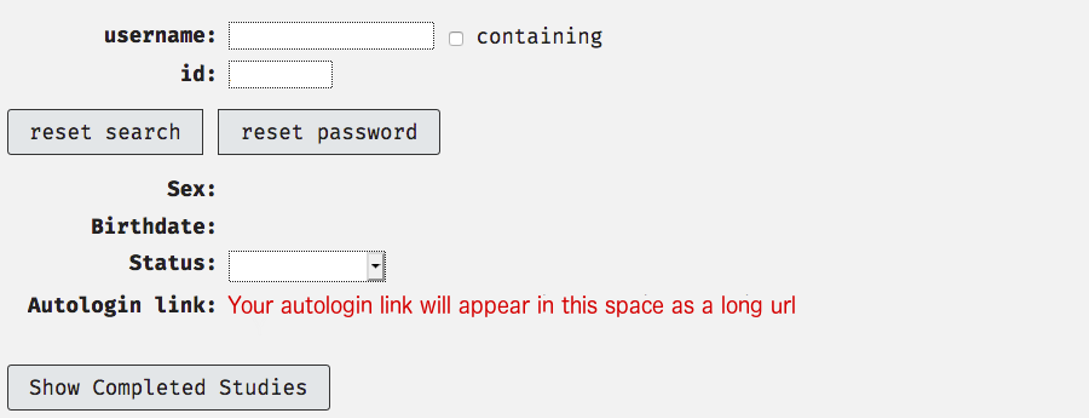
\includegraphics{images/screenshots/autologin.png}

Clicking on the autologin link will log you into the account of this user which allows you to examine what is going on in their account from the perspective of their account. This should be used for troubleshooting issues such as lack of access to the researchers section of the website and bugs that may be specific to their account or project(s).

These links are the same ones that the admins use to examine user accounts.

\hypertarget{appendices}{%
\chapter*{Appendices}\label{appendices}}
\addcontentsline{toc}{chapter}{Appendices}

\hypertarget{appendices-1}{%
\section*{Appendices}\label{appendices-1}}
\addcontentsline{toc}{section}{Appendices}

\hypertarget{commoncode}{%
\subsection*{Commonly Used R Code}\label{commoncode}}
\addcontentsline{toc}{subsection}{Commonly Used R Code}

\hypertarget{image-sources}{%
\subsection{Image Sources}\label{image-sources}}

All images original with the exception of the following:

\begin{itemize}
\tightlist
\item
  Rainbow Free Icon \citep{rainbow}
\item
  Tech Support Icon Pack \citep{techpack}
\item
  Traffic Cone Icon \citep{cone}
\end{itemize}

\hypertarget{software}{%
\subsection*{Software}\label{software}}
\addcontentsline{toc}{subsection}{Software}

This manual was written using R \citep{baser}, RStudio \citep{rstudio} and bookdown \citep{xie2015}.

Custom graphics created and screenshots edited with GIMP \citep{gimp}.

\hypertarget{references}{%
\section*{References}\label{references}}
\addcontentsline{toc}{section}{References}

\bibliography{book.bib,packages.bib}


\end{document}
